%% This is file `DEMO-TUDaBeamer.tex' version 3.10 (2021/02/22),
%% it is part of
%% TUDa-CI -- Corporate Design for TU Darmstadt
%% ----------------------------------------------------------------------------
%%
%%  Copyright (C) 2018--2021 by Marei Peischl <marei@peitex.de>
%%
%% ============================================================================
%% This work may be distributed and/or modified under the
%% conditions of the LaTeX Project Public License, either version 1.3c
%% of this license or (at your option) any later version.
%% The latest version of this license is in
%% http://www.latex-project.org/lppl.txt
%% and version 1.3c or later is part of all distributions of LaTeX
%% version 2008/05/04 or later.
%%
%% This work has the LPPL maintenance status `maintained'.
%%
%% The Current Maintainers of this work are
%%   Marei Peischl <tuda-ci@peitex.de>
%%   Markus Lazanowski <latex@ce.tu-darmstadt.de>
%%
%% The development respository can be found at
%% https://github.com/tudace/tuda_latex_templates
%% Please use the issue tracker for feedback!
%%
%% If you need a compiled version of this document, have a look at
%% http://mirror.ctan.org/macros/latex/contrib/tuda-ci/doc
%% or at the documentation directory of this package (if installed)
%% <path to your LaTeX distribution>/doc/latex/tuda-ci
%% ============================================================================
%%
% !TeX program = lualatex
%%

%% This is file `DEMO-TUDaBeamer.tex' version 3.10 (2021/02/22),
%% it is part of
%% TUDa-CI -- Corporate Design for TU Darmstadt
%% ----------------------------------------------------------------------------
%%
%%  Copyright (C) 2018--2021 by Marei Peischl <marei@peitex.de>
%%
%% ============================================================================
%% This work may be distributed and/or modified under the
%% conditions of the LaTeX Project Public License, either version 1.3c
%% of this license or (at your option) any later version.
%% The latest version of this license is in
%% http://www.latex-project.org/lppl.txt
%% and version 1.3c or later is part of all distributions of LaTeX
%% version 2008/05/04 or later.
%%
%% This work has the LPPL maintenance status `maintained'.
%%
%% The Current Maintainers of this work are
%%   Marei Peischl <tuda-ci@peitex.de>
%%   Markus Lazanowski <latex@ce.tu-darmstadt.de>
%%
%% The development respository can be found at
%% https://github.com/tudace/tuda_latex_templates
%% Please use the issue tracker for feedback!
%%
%% If you need a compiled version of this document, have a look at
%% http://mirror.ctan.org/macros/latex/contrib/tuda-ci
%% ============================================================================
%%
% !TeX program = lualatex
%%

\documentclass[
	%ngerman,%globale Übergabe der Hauptsprache
	aspectratio=169,%Beamer eigene Option zum Umschalten des Formates
	color={accentcolor=2d},
	logo=true,%Kein Logo auf Folgeseiten
	colorframetitle=true,%Akzentfarbe auch im Frametitle
%	logofile=example-image, %Falls die Logo Dateien nicht vorliegen
	]{tudabeamer}
\usepackage[]{babel}
\usepackage{iftex}
\ifPDFTeX
\usepackage[utf8]{inputenc}%kompatibilität mit TeX Versionen vor April 2018
\fi

%Makros für Formatierungen der Doku
%Im Allgemeinen nicht notwendig!
\let\code\texttt

\title{A Workflow for Increasing the Quality of Scientific Software\\ (in Computational Science and Engineering)}
\subtitle{Exascale Computing Project (ECP) IDEAS Productivity Webinar 2021-04-07}
\author[\textbf{T. Mari\'c}, JP. Lehr, I. Pappagianidis, B. Lambie, D. Bothe, C. Bischof]{Tomislav Mari\'c}
\department{TU Darmstadt, Germany}
\institute{CRC 1194 : Z-INF}

%Fremdlogo
%Logo Macro mit Sternchen skaliert automatisch, sodass das Logo in die Fußzeile passt
\logo*{
\includegraphics{./crc-logo}}

% Da das Bild frei wählbar nach Breite und/oder Höhe skaliert werden kann, werden \width/\height entsprechend gesetzt. So kann die Fläche optimal gefüllt werden.
%Sternchenversion skaliert automatisch und beschneidet das Bild, um die Fläche zu füllen.
%\titlegraphic*{\includegraphics{example-image}}
\titlegraphic{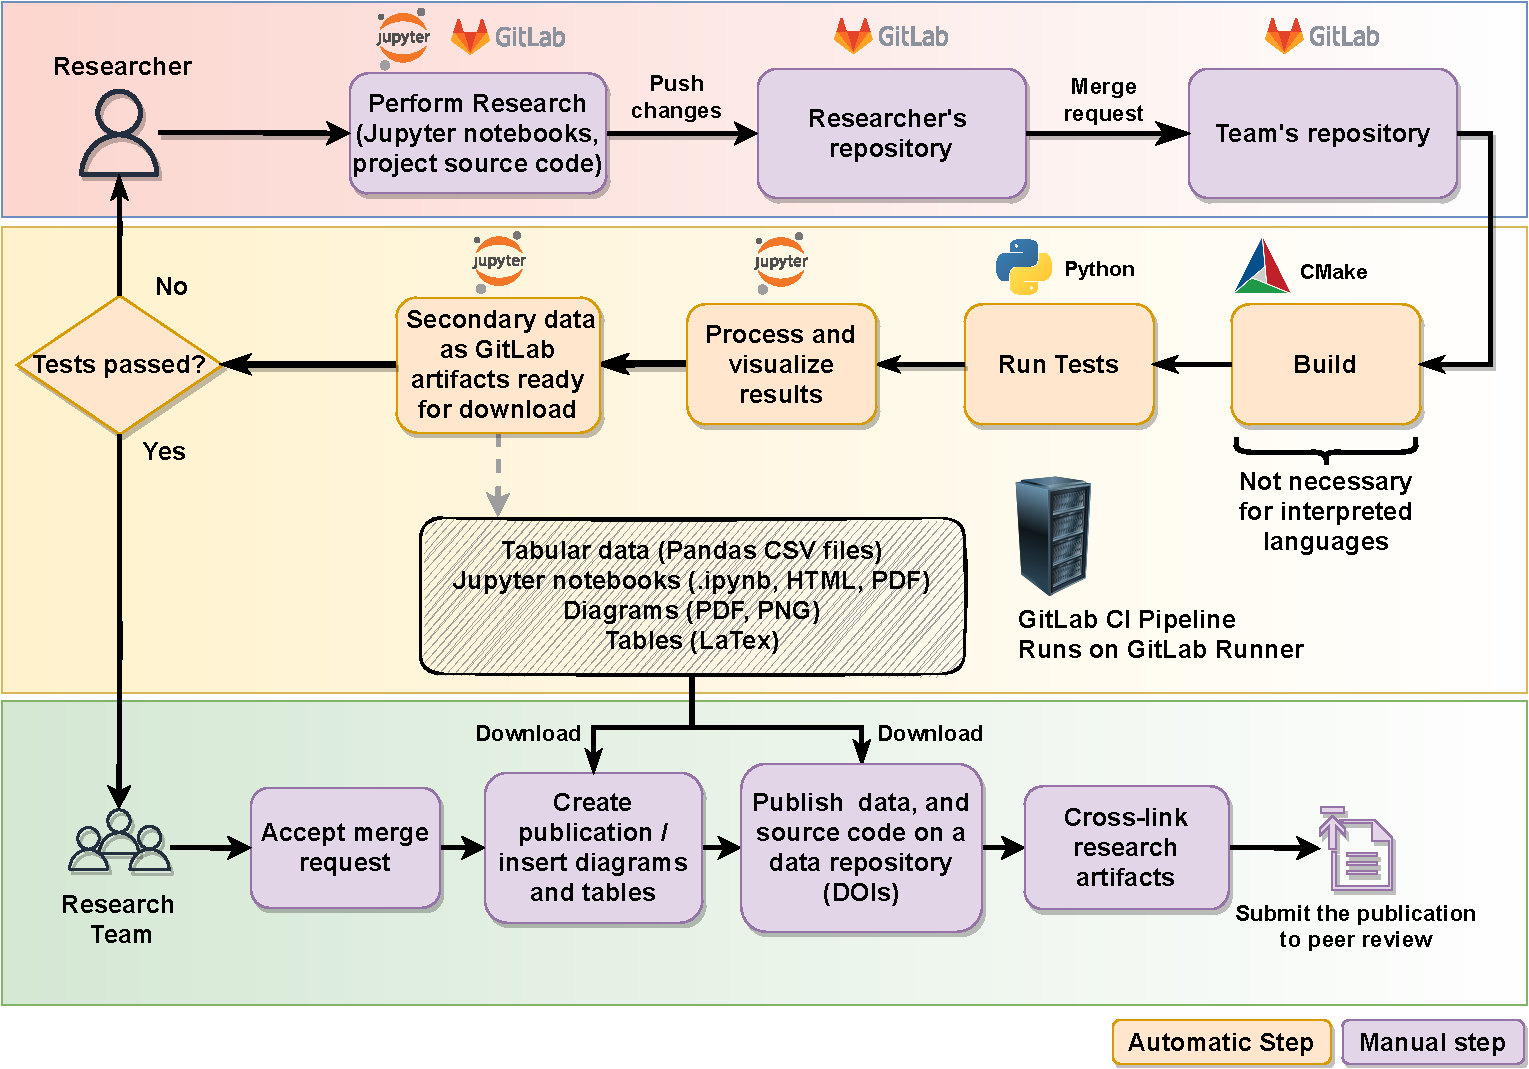
\includegraphics[scale=0.47]{figures/ZINF-CI-diagram.pdf}}
\date{ECP IDEAS Productivity Webinar 2021-04-07}

\usepackage{booktabs}
\usepackage{fontawesome}

\hypersetup{
  colorlinks,
  citecolor=violet,
  linkcolor=red,
  urlcolor=violet}

\begin{document}

\maketitle

\begin{frame}{Computational Science and Engineering software in\\university research groups}
	\framesubtitle{Boundary and initial conditions}
	
	\vfill
	\begin{itemize}
            \item Publish or perish \faGraduationCap\footnote{Symbol of a publish-or-perish simplification of the workflow :)} prioritizes publications over scientific software.
		\item Dedicated resources for increasing software quality are usually not available.
		\item Ph.D. students rotate every ~4-5 years, postdocs every 1-2 years. 
			\begin{itemize}
				\item Little or no overlap between successors and predecessors. 
			\end{itemize}
		\item Large-scale software design is not a necessary part of the CSE curriculum. 
			\begin{itemize}
				\item Different CSE background: (Applied) Mathematics, Mechanical Engineering, Physics, Informatics.
			\end{itemize}
		\item Real-world example: onboarding people into \href{https://www.openfoam.com/documentation/guides/latest/api/classes.html}{\beamergotobutton{OpenFOAM}} module development.
	\end{itemize}
\end{frame}

\begin{frame}{Computational Science and Engineering software in\\university research groups}
	\framesubtitle{Divergence}
	
	\vfill
	\begin{itemize}
            \item Not being able to continue development from an earlier state.
            \item Reproducing results from a publication is not possible.  
                \begin{itemize}
                    \item Data, source code and publication are not archived and cross-linked. 
                    \item The version used to generate the data is not documented. 
                \end{itemize}
            \item Not being able to re-use a model from a publication. 
                \begin{itemize}
                    \item The model is not implemented in a modular way.
                    \item Version integration was not done.
                    \item Non-granular commits were used. 
                \end{itemize}
            \item Having no overview of the impact of a change on the rest of the module.
	\end{itemize}

	\medskip

\end{frame}

%\begin{frame}{CSE software in the Collaborative Research Center 1194}

    %\begin{itemize}
        %\item OpenFOAM
    %\end{itemize}

%\end{frame}

\begin{frame}{A workflow for increasing the quality of scientific CSE software} 

    \vfill
    \begin{enumerate}
        \item Track the issues in a Kanban board. 
            \begin{itemize}
                \item Model issues as \href{https://betterscientificsoftware.github.io/PSIP-Tools/PTCs/}{Progress Tracking Cards}\footnote{Developed by \href{https://bssw.io/}{Better Scientific Software}}.
            \end{itemize}
        \item Use a simple version-control branching model. 
        \item Apply Test-Driven Development (TDD) for CSE software.
        \item Enable Continuous Integration with an emphasis on result visualization. 
        \item Cross-link software, result data, and report/article when reaching a milestone.
            \begin{itemize}
                \item When submitting a publication to peer-review. 
                \item After the publication has been accepted. 
                \item When giving up on an idea. 
            \end{itemize}
        \item Bonus step: publish a Singularity image with the code and data.
    \end{enumerate}
\end{frame}

\begin{frame}{A workflow for increasing the quality of (academic) CSE software} 
    \framesubtitle{OpenFOAM}

        \vfill

        The workflow is developed with OpenFOAM projects but it is tested with other software. 

        \vspace{1cm}

        \textbf{Disclaimer}: This offering is not approved or endorsed by OpenCFD Limited, producer and distributor of the OpenFOAM software via www.openfoam.com, and owner of the OPENFOAM®  and OpenCFD®  trade marks. 

\end{frame}

\begin{frame}{Simple version-control branching model} 
    \framesubtitle{Separation of Concerns and Single Responsibility}

	\vfill
	\begin{itemize}

            \item University research teams \emph{working on the same project} are generally small (2 - 5 members).
            \item \href{https://en.wikipedia.org/wiki/Separation_of_concerns}{\beamergotobutton{Separation of Concerns (SC)}} and \href{https://en.wikipedia.org/wiki/Single-responsibility_principle}{\beamergotobutton{Single Responsibility Principle (SRP)}} significantly simplify the branching model. 

            \item \textbf{Separation of Concerns}: code is organized in non-overlapping layers and sections. 

            \item \textbf{Single Responsibility}: functions or classes perform single clear tasks.

            \item SC and SRP can be applied to any software.
            \item Dogmatism should be avoided: single responsibility vs less responsibilities. 
            \item OpenFOAM already uses object-oriented and generic software design patterns.  

        \end{itemize}
\end{frame}

\begin{frame}{Simple version-control branching model} 
    \framesubtitle{Change integration}

        \vfill

        \textbf{Maintainers (postdocs, experienced Ph.D.\ students) manage the integration.} 

	\begin{itemize}
            \item Keep the branching model as simple as possible.  
            \item Main and development branches are protected and managed by Maintainers. 
            \item Maintainers are responsible for git tags and cleanup: 
            \begin{itemize}
                    \item \textbf{Main}: integrations from \emph{accepted publications} and \emph{development branch}. 
                    \item \textbf{Development}: integration of \emph{(CI)-tested improvements}. 
                    \item \textbf{Feature}: SRP reduces git-conflicts with researchers working on different files.
            \end{itemize}
            \item Complex branching workflow $\Rightarrow$ complications with onboarding new members.
	\end{itemize}

\end{frame}

\begin{frame}{Test Driven Development} 
    \framesubtitle{Program CSE tests first}
        \vfill


        TDD\footnote{Freeman, Steve, and Nat Pryce. Growing object-oriented software, guided by tests. Pearson Education, 2009.} for CSE
        \begin{itemize}
            \item Define verification and validation tests at the start.
            \item Focus placed the final result: interpolation, integration, discretization, PDE solution, physics. 
            \item Top-down, instead of bottom-up test coverage.
            \item Don't go overboard with unit-tests \faGraduationCap: extend unit-tests when debugging a failing CSE test.  
            \item Focus kept on tests with real-world (publication) input. 
        \end{itemize}

\end{frame}

\begin{frame}{Test Driven Development} 
    \framesubtitle{Verification and validation tests define the Application Programming Interface}
        \vfill

    \begin{itemize}
        \item \textbf{New code}: it is easier to program the API you wish for, if you are its first user. 
            \begin{itemize}
                \item Make the class interface easy to use correctly and difficult to use incorrectly\footnote{Scott Meyers. 2014. Effective Modern C++: 42 Specific Ways to Improve Your Use of C++11 and C++14 (1st. ed.). O'Reilly Media, Inc.}.
                \item Reduce number of function arguments, single responsibility, clear naming, ... 
            \end{itemize}
        \item \textbf{Legacy code}: extend existing API without modification. 
            \begin{itemize}
                \item OpenFOAM: understanding class hierarchies, \textit{finding a base class with Runtime Type Selection and a virtual function to overload.}
            \end{itemize}
        \item \textbf{The test application is the solver application with a different input.}
            \begin{itemize}
                \item If possible, testing and solution is done by the same code.  
                \item This prevents code duplication. 
                \item Data output and additional checks can be disabled by (compile-time) options.
            \end{itemize}
    \end{itemize}

\end{frame}


\begin{frame}{Test Driven Development} 
    \framesubtitle{Jupyter notebooks}

    \vfill
    Jupyter notebooks 
    \begin{itemize}
        \item \textbf{Documentation}: geometry, initial and boundary conditions, error norms, comparison data.
        \item \textbf{Processing}: verification errors (conservation, convergence, stability), validation errors. 
        \item \textbf{Result analysis}: very straightforward, interactive, remote.
    \end{itemize}
\end{frame}

\begin{frame}{Test Driven Development} 
    \framesubtitle{Parameter tests}
    
    \vfill
    \begin{center}
            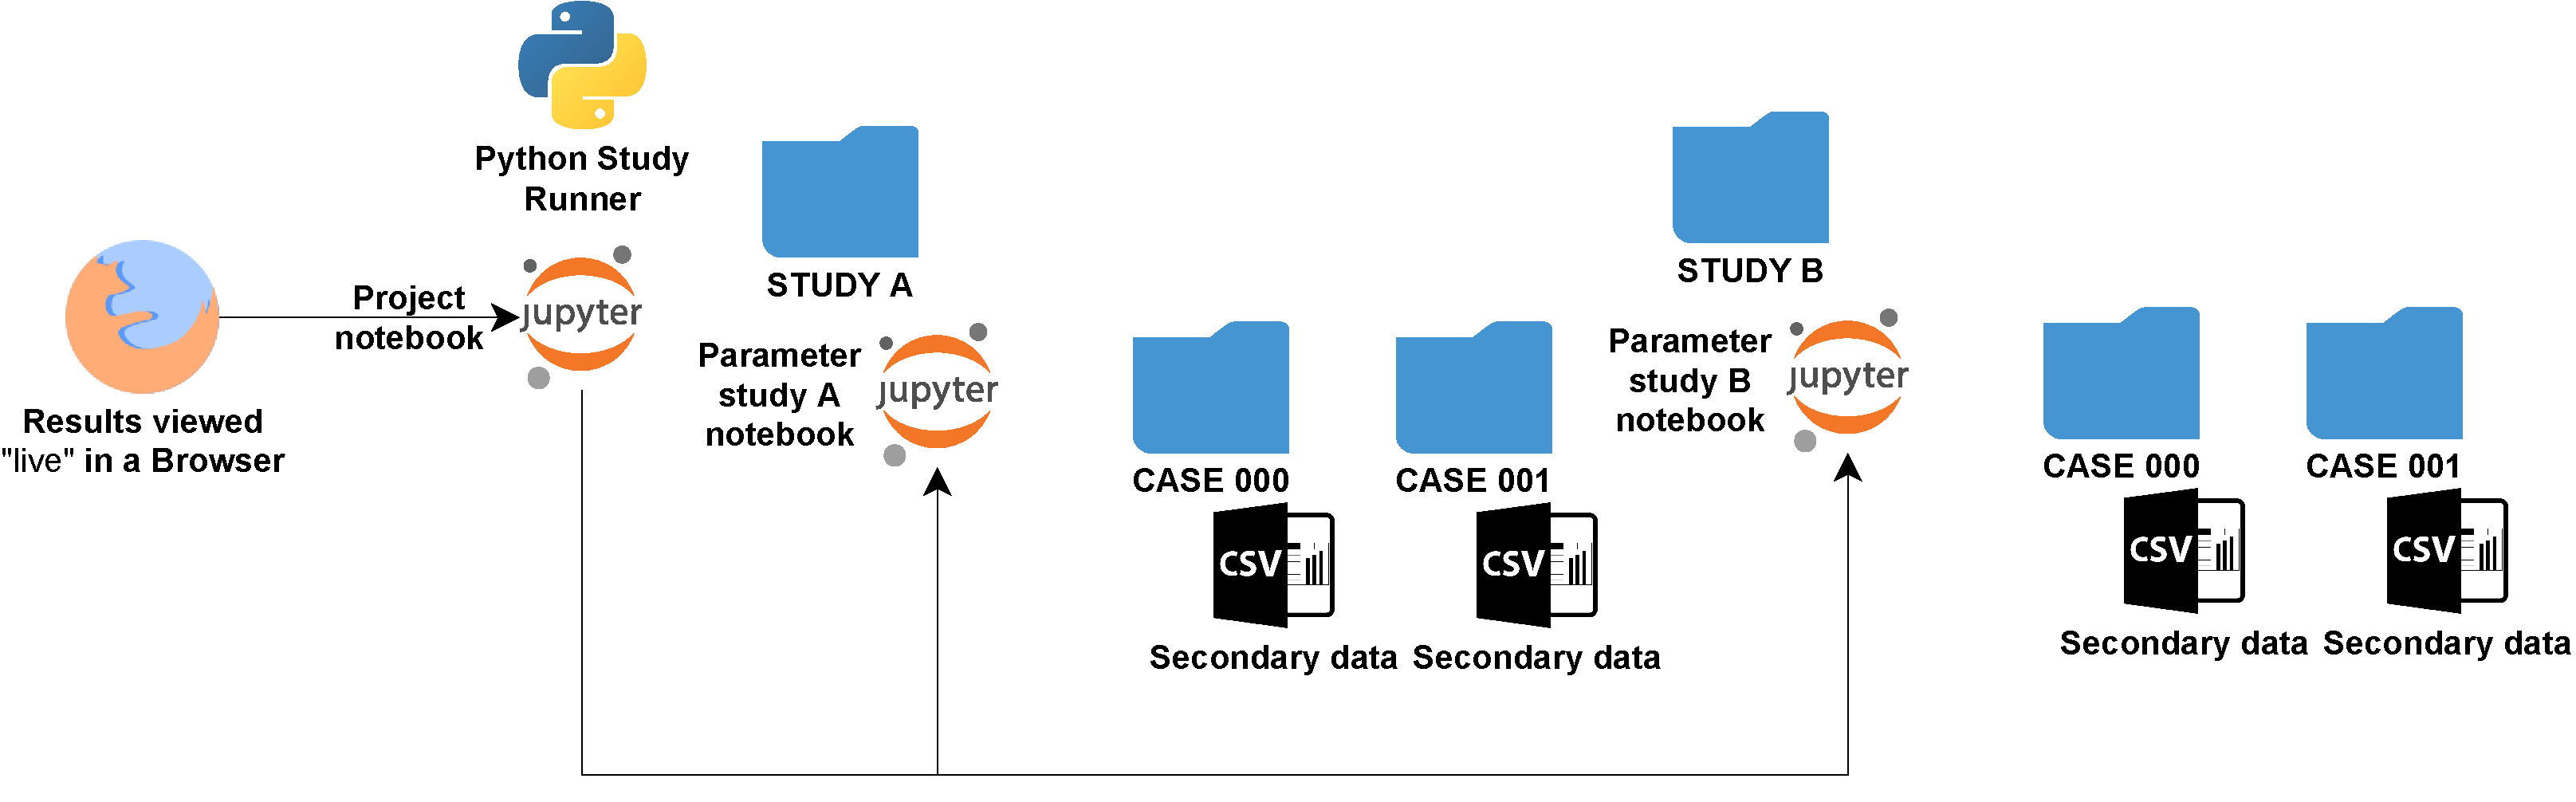
\includegraphics[width=0.9\textwidth]{figures/Cluster-Parameter-Study-Organization.pdf}
    \end{center}
\end{frame}

\begin{frame}{Test Driven Development} 
    \framesubtitle{Parameter tests: primary data (simulation results) organization}

    \begin{itemize}
        \item The quality of CSE software is measured using verification and validation data. 
        \item Effective comparison with others (previous versions) hinges on data organization.
    \end{itemize}
    
    \vfill
    \begin{itemize}
        \item \textbf{Legacy code primary data}: 
            \begin{itemize}
                \item use the existing folder structure and parameterization tools \faGraduationCap,
                \item The mapping (caseXYZ) $\to$ (parameter vector) must be stored (YAML, ...)
            \end{itemize}
        \item \textbf{New code primary data options}: 
            \begin{enumerate}
                \item Same as legacy code \faGraduationCap
                \item HDF5\footnote{\url{https://www.hdfgroup.org/solutions/hdf5}} or other open data format.
                \item Alternative to HDF5: \textbf{ExDir}\footnote{Dragly, Svenn-Arne, et al. "Experimental Directory Structure (Exdir): An alternative to HDF5 without introducing a new file format." Frontiers in neuroinformatics 12 (2018): 16.} 
            \end{enumerate}
    \end{itemize}

\end{frame}


\begin{frame}{Test Driven Development} 
    \framesubtitle{Parameter tests: secondary data (tables and diagrams) organization}

    \texttt{pandas.MultiIndex} CSV with metadata for secondary data
    \begin{itemize}
        \item \texttt{pandas.MultiIndex} saved in "metadata columns". 
        \item \textcolor{red}{\textbf{Metadata is repeated}}: not an issue for the small secondary data! 
        \item Metadata in columns $\to$ \texttt{pandas.MultiIndex} $\to$ strongly simplified data analysis. 
        \item \textbf{Direct readable export of tables to LaTex!}
    \end{itemize}

    \footnotesize

    \begin{tabular}{lllrrr}
        \toprule
        {} &         H &     L\_INF &  O(L\_INF) &  EPSILON\_R\_EXACT\_MAX &  O(EPSILON\_R\_EXACT\_MAX)  \\ 
        VELOCITY\_MODEL &           &           &           &                      &                        \\ 
        \midrule
        \textcolor{red}{\textbf{SHEAR\_2D}}       &  0.125000 &  0.032961 &  1.833407 &             0.032961 &                1.833407 \\ 
        \textcolor{red}{\textbf{SHEAR\_2D}}       &  0.062500 &  0.009249 &  1.955529 &             0.009249 &                1.955529 \\ 
        \textcolor{red}{\textbf{SHEAR\_2D}}       &  0.031250 &  0.002385 &  1.988745 &             0.002385 &                1.988745 \\ 
        \textcolor{red}{\textbf{SHEAR\_2D}}       &  0.015625 &  0.000601 &  1.997178 &             0.000601 &                1.997178 \\ 
        \textcolor{red}{\textbf{SHEAR\_2D}}       &  0.007813 &  0.000150 &  1.999294 &             0.000150 &                1.999294 \\ 
        \textcolor{red}{\textbf{SHEAR\_2D}}       &  0.003906 &  0.000038 &  1.999294 &             0.000038 &                1.999294 \\ 
        \bottomrule
    \end{tabular}

\end{frame}

\begin{frame}{Continuous Integration with result visualization} 
	\framesubtitle{Schematic diagram}

	\centering
	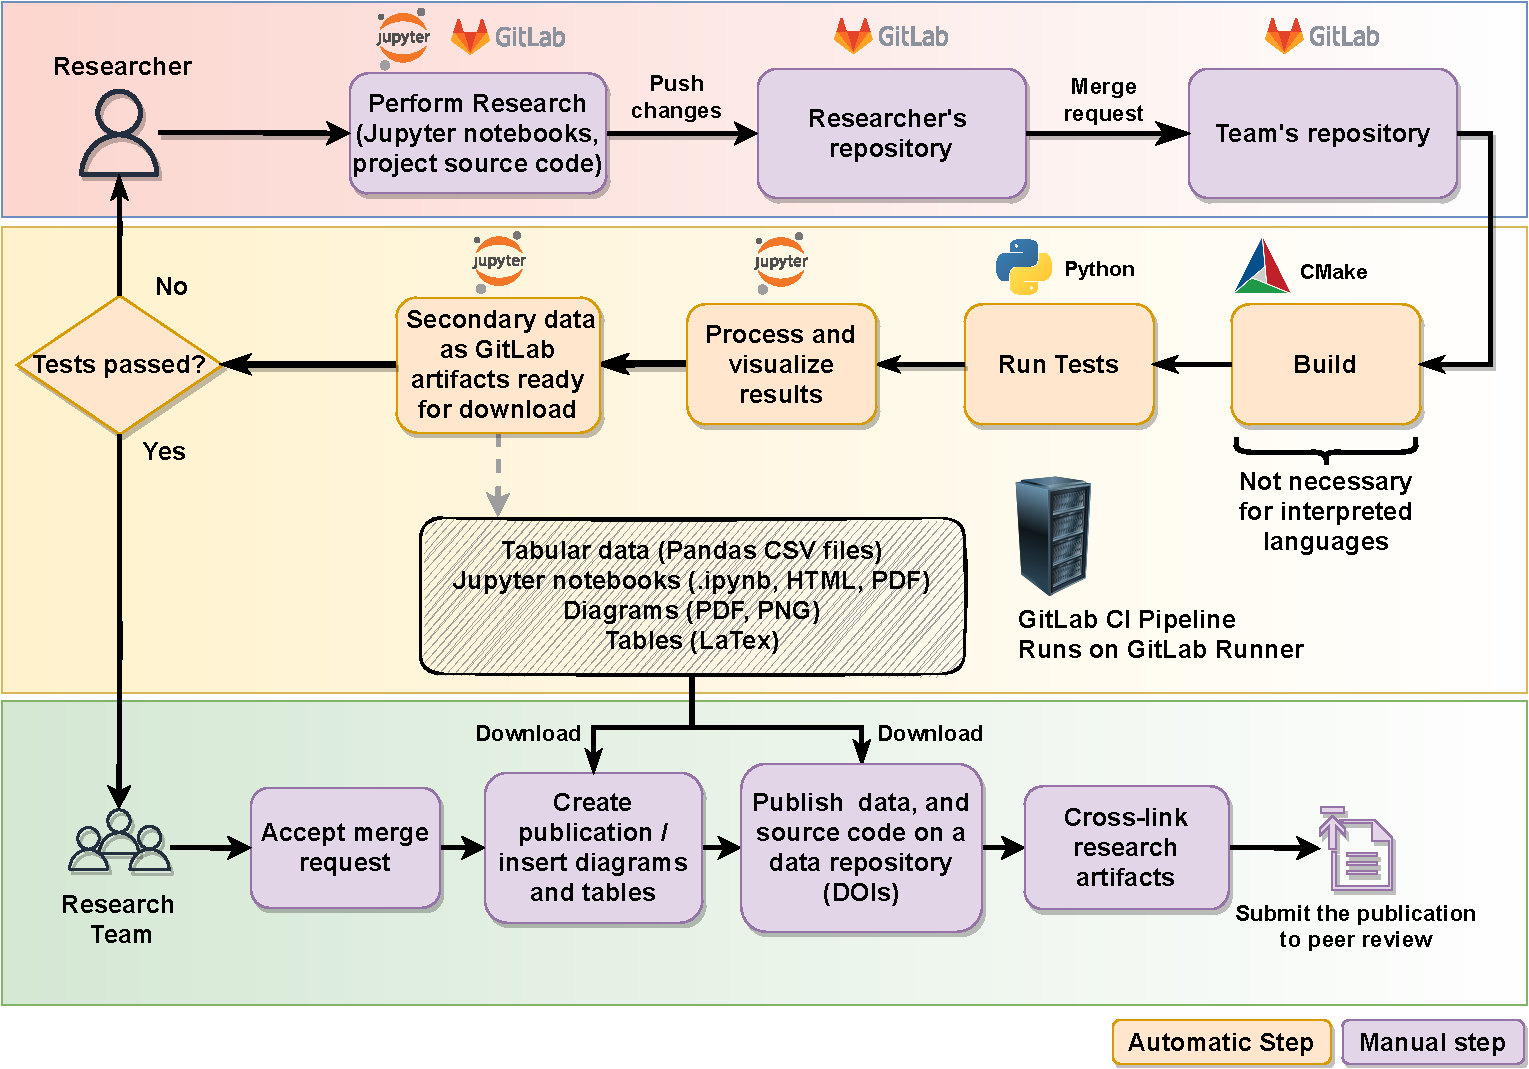
\includegraphics[width=0.8\textwidth]{figures/ZINF-CI-diagram.pdf}

\end{frame}

\begin{frame}{Continuous Integration with result visualization} 
    \framesubtitle{Testing machines and test categorization}

    \vfill
    \begin{enumerate}
        \item \textbf{Short few CPU-core tests}: work-PC \faGraduationCap.    
        \item \textbf{Short many-core tests}: obtain a workstation with a 64-Core CPU\footnote{Thanks to \href{https://www.sfb1194.tu-darmstadt.de/index.en.jsp}{CRC 1194 at TU Darmstadt.}}\faGraduationCap.
        \item \textbf{HPC tests}: combine 1. or 2. with an HPC cluster. 
    \end{enumerate}

    An HPC cluster is relevant for production tests and performance measurements.
    \begin{itemize}
        \item This workflow uses coarse ("smoke") tests \faGraduationCap
            \begin{itemize}
                \item Unit tests run for 1. and 2.
                \item Convergence ensured for 1. and 2.
                \item Is efficient in parallel for 1. and 2. 
            \end{itemize}
        \item \textbf{Challenge}: Is it possible to combine 1., 2. and 3. and publish instead of perish \faGraduationCap?
    \end{itemize}

\end{frame}


\begin{frame}{Continuous Integration with result visualization} 
    \framesubtitle{A GitLab runner with a Docker executor and a local Docker image}

    \vfill 
    Build a Docker image for your software, and track the Dockerfile with the project.\\
    \medskip
    \href{https://gitlab.com/tmaric/fvc-reconstruct/-/tree/main/docker}{Example OpenFOAM Dockerfile} on \texttt{ubuntu:focal} with "system" open-mpi and scotch.

    \medskip
    On the testing machine
    \begin{itemize}
        \item Install Docker and GitLab runner and register the GitLab runner with a Docker executor.
        \item Configure the GitLab runner in \texttt{/etc/gitlab-runner/config.toml} to
            \begin{itemize}
                \item use a local Docker image, e.g., \texttt{image = "openfoam-v2012\_ubuntu:focal"}, and
                \item never pull images \texttt{pull\_policy = never}.
            \end{itemize}
    \end{itemize}


\end{frame}

\begin{frame}{Continuous Integration with result visualization} 
    \framesubtitle{Building}

    \vfill
    \begin{itemize}
        \item Files created within a job are gone when the job ends. 
        \item GitLab uses \textbf{job artifacts} to pass on data from one job to the next. 
        \item \textbf{Job artifacts only work with files stored in project's sub-folders.} 
        \item Libraries and applications are passed to other jobs as artifacts. 
        \item Artifacts can be downloaded on the GitLab project website.  
    \end{itemize}

\end{frame}

\begin{frame}[fragile]{Continuous Integration with result visualization} 
    \framesubtitle{Building OpenFOAM projects or projects with out-of-source installation}

    \vfill
    \textbf{Out-of-source installation}: binaries only available outside the repo! 
    \begin{itemize}
        \item \textbf{Use environment variables to build and pass on artifacts} 
        \item \texttt{\$FOAM\_USER\_LIBBIN} folder stores library binaries. 
        \item \texttt{\$FOAM\_USER\_APPBIN} folder stores application binaries. 
        \item \textbf{Build job}: 
            \begin{itemize}
                \item create artifact folders inside the repo, 
                \item copy library and application binaries to artifact folders, 
                \item export artifact folders. 
            \end{itemize}
        \item \textbf{Run job}: 
            \begin{itemize} 
                \item \texttt{mkdir -p} \texttt{{\$FOAM\_USER\_LIBBIN, \$FOAM\_USER\_LIBBIN}}
                \item Copy binaries from the artifact folders to \texttt{\$FOAM\_USER\_LIBBIN} and  \texttt{\$FOAM\_USER\_APPBIN} 
                \item Run tests.
            \end{itemize}
    \end{itemize}


\end{frame}

\begin{frame}{Continuous Integration with result visualization} 
	\framesubtitle{Schematic diagram}

	\centering
	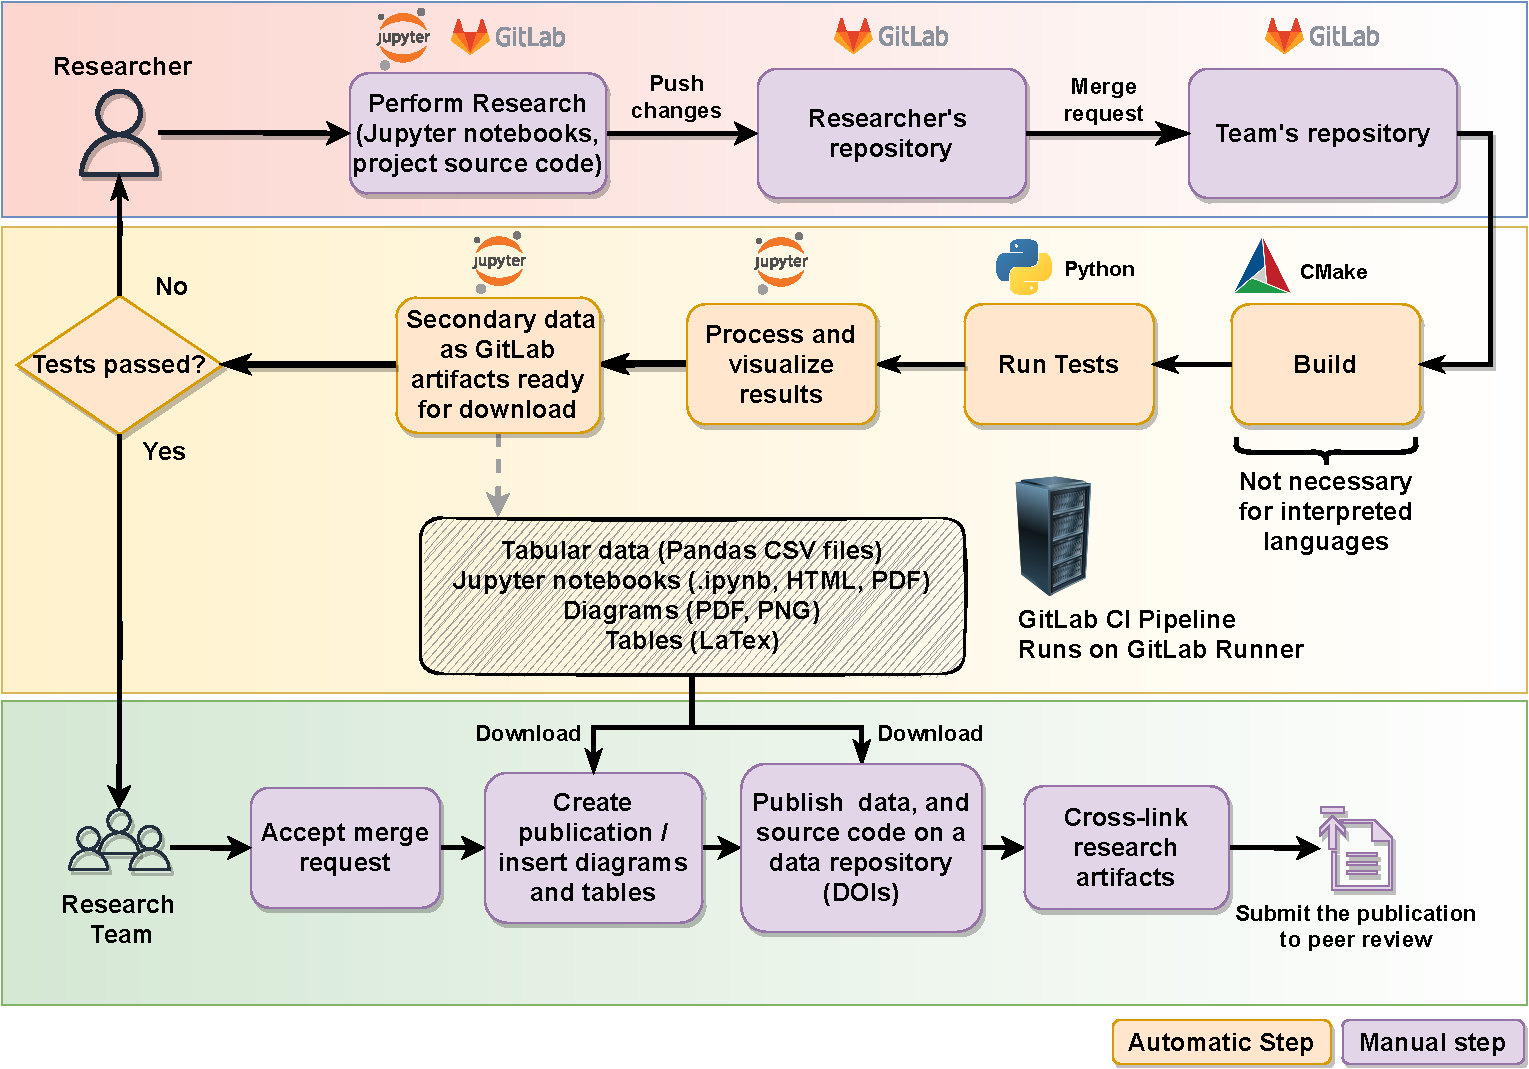
\includegraphics[width=0.8\textwidth]{figures/ZINF-CI-diagram.pdf}

\end{frame}

\begin{frame}{Continuous Integration with result visualization} 
    \framesubtitle{Processing and visualizing results}

    \vfill

    \texttt{jupyter nbconvert notebook.ipynb --execute --to FORMAT}

    \medskip

    \begin{itemize}
        \item Execute each jupyter notebook in the repository.
        \item Notebooks agglomerate secondary data into \texttt{pandas.MultiIndex} CSV files. 
        \item Export secondary data and notebooks in different formats as artifacts.
        \item \textbf{Visualization} 
            \begin{itemize}
                \item Download the artifact and open the notebook \faGraduationCap.
                \item \textbf{Alternative:} publish the notebook as a blog post in a GitLab Static Page project. 
                \item Notebooks contain information on failing tests. 
                \item Mapping "caseXYZ" $\to$ "parameter vector" is crucial for re-starting failed parameter variations! 
            \end{itemize}
    \end{itemize}

\end{frame}


\begin{frame}{Continuous Integration with result visualization} 
    \framesubtitle{Test evaluation}

    \vfill

    Very simple
    \begin{itemize}
        \item Python scripts that test secondary data agglomerated by the notebooks from simulation results.
        \item \textbf{Examples:} 
            \begin{itemize}
                \item Is the order of convergence of an error norm $\ge 2.0$?
                \item Is is the difference between simulation and experiment data $\le 4\%$? 
            \end{itemize}
    \end{itemize}

\end{frame}

\begin{frame}{Continuous Integration with result visualization} 
    \framesubtitle{Example}

    \vfill
    \begin{center}
        \href{https://gitlab.com/tmaric/fvc-reconstruct/-/pipelines/276526868}{Example OpenFOAM CI project} 
    \end{center}

\end{frame}

\begin{frame}{Cross-linking data, source code and reports/publications} 
	\framesubtitle{Schematic diagram}
	
	\begin{center}
		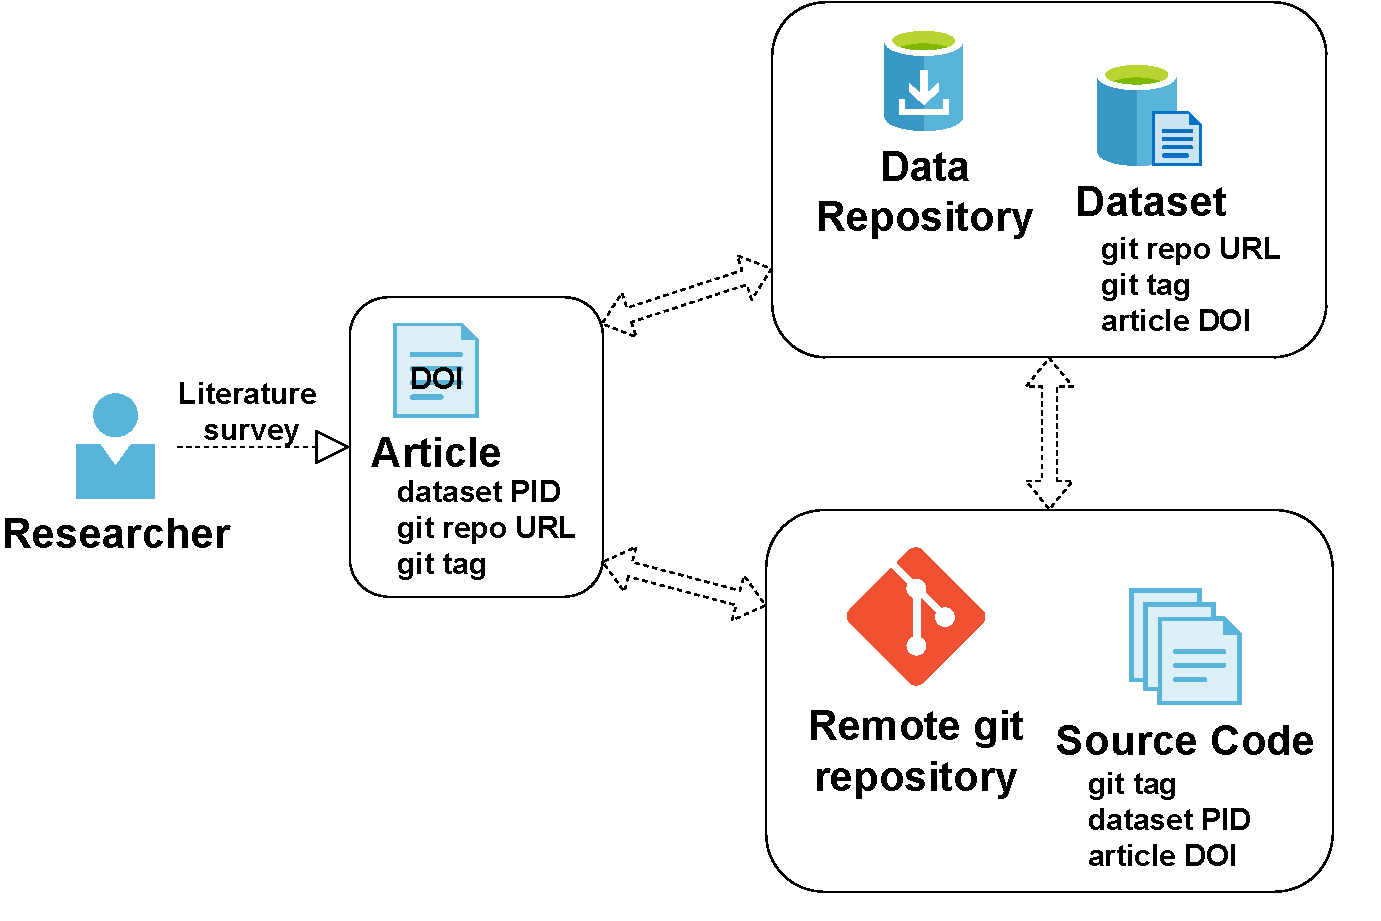
\includegraphics[width=0.67\textwidth]{figures/cross-linking.pdf}
	\end{center}

\end{frame}

\begin{frame}{Cross-linking data, source code and reports/publications} 
    \framesubtitle{Singularity} 
        
    \vfill
    \begin{itemize}
        \item Whence the Singularity Image\footnote{https://sylabs.io/docs/}?
            \begin{itemize}
                \item More inutitive than Docker: \textbf{a Singularity image is a file.} 
                \item Built for HPC from the start. 
                \item Doesn't require root rights. 
                \item Easily reproducing results as \emph{actual files on a disk}, not "stuff in spinning containers". 
                \item Maps user folder to the container: result data remains on the host. 
            \end{itemize}
        \item Why not replace Docker with Singularity within GitLab CI? 
            \begin{itemize}
                \item We're learning how to do this using \href{https://docs.gitlab.com/runner/executors/custom.html}{GitLab custom executors}.
                \item Does the workflow still survive publish-or-perish \faGraduationCap test?
            \end{itemize}
        \item Why a source-code snapshot on-top of the image and the repository? 
            \begin{itemize}
                \item Repositories get migrated, deleted, and some researchers still fear images. 
                \item Quick and direct access to source code from the publication. 
            \end{itemize}
    \end{itemize}

\end{frame}

\begin{frame}{Cross-linking data, source code and reports/publications} 
    \framesubtitle{Singularity simplifies reproducibility}

    \begin{itemize}
        \item The source code and the data stored in the image can be quickly reproduced.
        \item Article reviewers can clone, build, run and visualize easily. 
    \end{itemize}

    \href{https://git.rwth-aachen.de/leia/geophase/-/blob/JCOMP-D-19-01329R2/geophase.def}{Example: Singularity Image from an active review}
    \begin{itemize}
        \item Clone the code repository from the image: \\ \texttt{geophase-JCOMP-D-19-01329R2.sif clone geophase}
        \item Build: \\ \texttt{geophase-JCOMP-D-19-01329R2.sif build geophase build}
        \item Run tests: \\ \texttt{geophase-JCOMP-D-19-01329R2.sif run-tests geophase build}
        \item Open the jupyter notebook: \\ \texttt{geophase-JCOMP-D-19-01329R2.sif jupyter-notebook geophase}
    \end{itemize}

\end{frame}


%\begin{frame}{Cross-linking data, source code and reports/publications} 
	
	%\vfill
	%\begin{itemize}
		%\item Archive secondary data on a data repository (DOI). 
		%\item Archive primary data on a data repository (DOI). 
		%\item Create a git tag on the remote git repository. 
		%\item Archive the source code, binaries and secondary data in a Singularity container (DOI). 
		%\item Refer to result data DOIs, the git repo and the tag in the publication.
		%\item Upload the publication to a repository (DOI, arXiv-ID).
			%\begin{itemize}
				%\item For tech reports and milestones, DOIs can be requested without publication.
			%\end{itemize}
		%\item Edit metadata and the git-tag description until everything is cross-linked.
	%\end{itemize}

%\end{frame}

\begin{frame}{Similarity with other workflows / best practices}

	\vfill
	Our \emph{(subjective)} estimates* of similarity $1-5$ (higher is more similar), $-$: aspect not addressed.
	\begin{center}
		\scriptsize
		\begin{tabular}{@{} *6l @{}}    \toprule
				\emph{DOI} & \emph{Branching model} & \emph{TDD} & \emph{Cross-linking} & \emph{CI}  & (Meta)data standardization \\\midrule
				 \href{https://doi.org/10.12688/f1000research.11407.1}{10.12688/f1000research.11407.1} 
					 & -  & -  & -  & - & 1  \\ 
				 \href{https://doi.org/10.3934/math.2016.3.261}{10.3934/math.2016.3.261} 
					 & -  & -  & -  & - & 2  \\ 
				 \href{https://doi.org/10.1371/journal.pbio.1001745}{10.1371/journal.pbio.1001745} 
					 & 1  & 2  & -  & - & -  \\ 
				 \href{https://doi.org/10.1371/journal.pcbi.1005510}{10.1371/journal.pcbi.1005510}
					 & -  & -  & 3 & 1 & 3  \\ 
				 \href{https://doi.org/10.1145/2723872.2723881}{10.1145/2723872.2723881}
					 & 1  & -  & - & 1 & -  \\ 
				 \href{https://dl.acm.org/doi/10.1145/3324989.3325719}{10.1145/3324989.3325719}
					 & 1  & -  & - & 5 & -  \\ 
				 \href{https://doi.org/10.1371/journal.pone.0230557}{10.1371/journal.pone.0230557}
					 & 1  & -  & - & 1 & 4  \\ 
				 \href{https://doi.org/10.1145/3219104.3219147}{10.1145/3219104.3219147} 
					 & 1  & -  & -  & 4 & - \\\bottomrule
				 \hline
		\end{tabular}
	\end{center}
	
	*\emph{The list may still be incomplete.}
	
\end{frame}

\begin{frame}{Outlook}
	\vfill
	\begin{itemize}
            \item Performance CI jobs run on 64-core workstations: moving on to the HPC cluster. 
            \item Singularity GitLab executor? 
            \item Jupyter Hub for interactive analysis of problems in parameter variations?
            \item Automatic publishing and cross-linking of CI artifacts? 
                \begin{itemize}
                    \item Source code archive, Singularity container, secondary data. 
                    \item Data repository API must be used to modify metadata. 
                \end{itemize}
	\end{itemize}
\end{frame}

\begin{frame}{Acknowledgements}

	\vfill
	{\
		Funded by the German Research Foundation (DFG) – Project-ID 265191195 – SFB 1194 : Z-INF
	}

\end{frame}

\end{document}

